\documentclass[final]{beamer}
\usepackage[orientation=portrait,size=a1,scale=1.2]{beamerposter}
\usepackage[utf8]{inputenc}
\usepackage[czech]{babel}
\usepackage{amsmath,amssymb}
\usepackage{booktabs}
\usepackage{graphicx}
\usepackage{xcolor}

% =========================================================================
% OFICIÁLNÍ BAREVNÁ PALETA FAV ZČU
% =========================================================================
\definecolor{favBlue}{RGB}{0, 90, 156}        % Oficiální modrá ZČU/FAV
\definecolor{favYellow}{RGB}{243, 146, 0}      % Akcentní žlutá FAV
\definecolor{favBgLight}{RGB}{246, 248, 251}   % Světlé pozadí bloků
\definecolor{textDark}{RGB}{30, 30, 30}

\setbeamercolor{headline}{bg=favBlue,fg=white}
\setbeamercolor{block title}{bg=favBlue,fg=white}
\setbeamercolor{block body}{bg=favBgLight,fg=textDark}
\setbeamercolor{structure}{fg=favBlue}

\setbeamertemplate{navigation symbols}{}
\setbeamertemplate{caption}[numbered]

% =========================================================================
% HLAVIČKA POSTERU — ČISTĚ FAV ZČU
% =========================================================================
\setbeamertemplate{headline}{
  \leavevmode
  \begin{beamercolorbox}[wd=\paperwidth,sep=1.4cm]{headline}
    \begin{columns}[c]
      \begin{column}{0.72\paperwidth}
        \vskip0.5ex
        {\LARGE \textbf{Úloha 1: Vícerozměrné náhodné veličiny}}\\[0.8ex]
        {\large \textbf{Generování dat a teoretické charakteristiky sdruženého rozdělení}}\\[1.6ex]
        \normalsize
        \textbf{Autoři:} Daniel Štefan, Matyáš Matějka \\
        \small Katedra matematiky (KMA), Fakulta aplikovaných věd, Západočeská univerzita v Plzni \\
        Předmět: Mnohorozměrné statistické metody (KMA/MSM)
      \end{column}
      \begin{column}{0.23\paperwidth}
        \raggedleft
        
\includegraphics[width=\linewidth]{img/kma-cmyk-cz.pdf}
      \end{column}
    \end{columns}
    \vskip0.5ex
  \end{beamercolorbox}
  \vspace{-1pt}
  \textcolor{favYellow}{\rule{\paperwidth}{7pt}} % Žlutý akcentní proužek FAV
}

\pdfmapfile{+sansmathaccent.map}

\begin{document}
\begin{frame}[t]

\vspace{0.4cm}

\begin{columns}[t]

% =========================================================================
% LEVÝ SLOUPEC: TEORETICKÁ ČÁST
% =========================================================================
\begin{column}{0.48\textwidth}

  % 1. Blok: Zadání a určení konstanty
  \begin{block}{1. Zadání a určení normalizační konstanty $c$}
    Uvažujeme sdruženou hustotu pravděpodobnosti náhodného vektoru $(X, Y)$:
    \[
      f(x, y) = c \cdot \cos(y - x) \quad \text{na oblasti } \Omega = \left\{ (x, y) \in \mathbb{R}^2;\, 0 \le x \le \frac{\pi}{2},\, x \le y \le \frac{\pi}{2} \right\}.
    \]
    Konstantu $c$ určíme z podmínky $\iint_\Omega f(x, y) \, \mathrm{d}x \, \mathrm{d}y = 1$:
    \[
      c \int_0^{\pi/2} \left( \int_0^y \cos(y - x) \, \mathrm{d}x \right) \mathrm{d}y = 1.
    \]
    \begin{itemize}
      \item Vnitřní integrál: $\displaystyle\int_0^y \cos(y - x) \, \mathrm{d}x = \big[ -\sin(y - x) \big]_{x=0}^{x=y} = \sin(y)$.
      \item Vnější integrál: $\displaystyle\int_0^{\pi/2} \sin(y) \, \mathrm{d}y = \big[ -\cos(y) \big]_0^{\pi/2} = 1 \implies \mathbf{c = 1}$.
    \end{itemize}
    Platná hustota je tedy $f(x, y) = \cos(y - x)$ na trojúhelníku $\Omega$.
    \begin{center}
      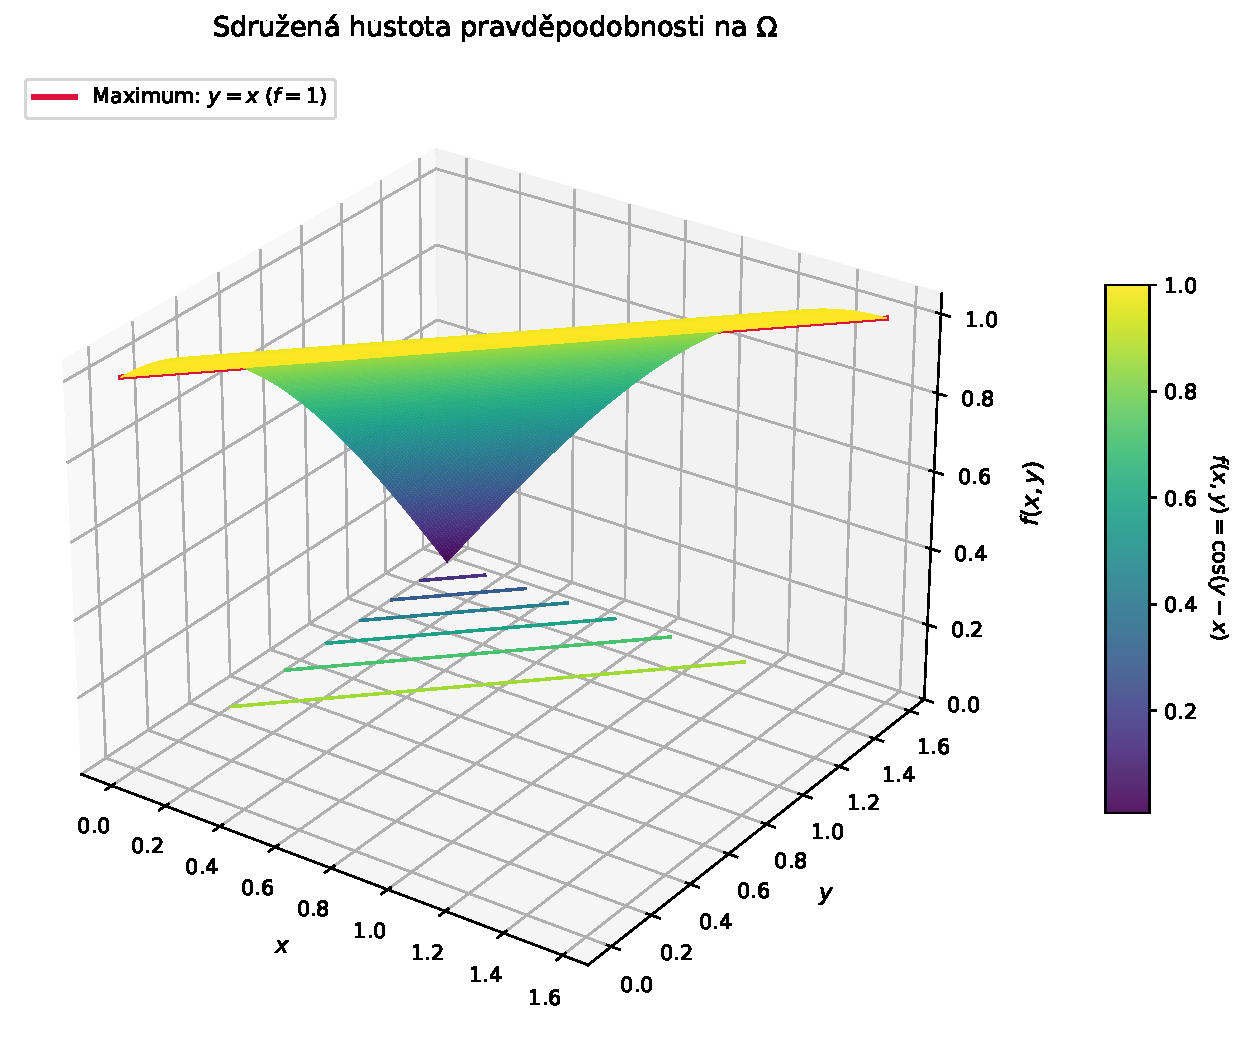
\includegraphics[width=0.78\textwidth]{img/graf_funkce.pdf}
    \end{center}
  \end{block}

  \vskip1.5ex

  % 2. Blok: Marginální rozdělení
  \begin{block}{2. Marginální hustoty a distribuční funkce}
    Marginální hustoty získáme vyintegrováním druhé proměnné přes nosič:
    \begin{itemize}
      \item \textbf{Pro složku $X$ ($x \in [0, \pi/2]$):}
      \[
        f_X(x) = \int_x^{\pi/2} \cos(y - x) \, \mathrm{d}y = \big[\sin(y - x)\big]_{y=x}^{\pi/2} = \mathbf{\cos(x)}.
      \]
      \item \textbf{Pro složku $Y$ ($y \in [0, \pi/2]$):}
      \[
        f_Y(y) = \int_0^y \cos(y - x) \, \mathrm{d}x = \big[-\sin(y - x)\big]_{x=0}^y = \mathbf{\sin(y)}.
      \]
    \end{itemize}
    Marginální distribuční funkce integrací příslušných hustot pro $x, y \in [0, \pi/2]$:
    \[
      F_X(x) = \int_0^x \cos(t) \, \mathrm{d}t = \mathbf{\sin(x)}, \qquad
      F_Y(y) = \int_0^y \sin(t) \, \mathrm{d}t = \mathbf{1 - \cos(y)}.
    \]
  \end{block}

  \vskip1.5ex

  % 3. Blok: Teoretické charakteristiky
  \begin{block}{3. Teoretické charakteristiky a variační matice}
    \textbf{Střední hodnoty:}
    \[
      E(X) = \int_0^{\pi/2} x \cos(x) \, \mathrm{d}x = \frac{\pi - 2}{2} \approx 0{,}5708, \quad
      E(Y) = \int_0^{\pi/2} y \sin(y) \, \mathrm{d}y = 1.
    \]
    \textbf{Rozptyly:}
    \[
      \operatorname{var}(X) = E(X^2) - [E(X)]^2 = \left(\frac{\pi^2}{4} - 2\right) - \left(\frac{\pi - 2}{2}\right)^2 = \mathbf{\pi - 3} \approx 0{,}1416,
    \]
    \[
      \operatorname{var}(Y) = E(Y^2) - [E(Y)]^2 = (\pi - 2) - 1^2 = \mathbf{\pi - 3} \approx 0{,}1416.
    \]
    \textbf{Kovariance a variační matice:}
    \[
      E(XY) = \int_0^{\pi/2} \int_0^y x y \cos(y - x) \, \mathrm{d}x \, \mathrm{d}y = 1 - \frac{\pi}{2} + \frac{\pi^2}{8},
    \]
    \[
      \operatorname{cov}(X, Y) = E(XY) - E(X)E(Y) = \frac{\pi^2}{8} - \pi + 2 \approx 0{,}0921.
    \]
    \[
      \mathbf{\Sigma} = \begin{pmatrix} \operatorname{var}(X) & \operatorname{cov}(X, Y) \\ \operatorname{cov}(X, Y) & \operatorname{var}(Y) \end{pmatrix} 
      \approx \begin{pmatrix} 0{,}1416 & 0{,}0921 \\ 0{,}0921 & 0{,}1416 \end{pmatrix}.
    \]
  \end{block}

\end{column}


% =========================================================================
% PRAVÝ SLOUPEC: EXPERIMENTÁLNÍ ČÁST (SIMULACE A GRAFY)
% =========================================================================
\begin{column}{0.48\textwidth}

  % 4. Blok: Generování dat
  \begin{block}{4. Generování dat (Zamítací metoda)}
    Kandidáti $(X, Y)$ jsou generováni z rovnoměrného 2D rozdělení na čtverci $[0, \pi/2]^2$ s hustotou $g(x, y) = 4/\pi^2$. Obálková konstanta je $M = \pi^2/4 \approx 2{,}467$.
    Bod je přijat, pokud $x \le y$ a platí $v \le \cos(y - x)$ pro $v \sim U(0, 1)$. Teoretická pravděpodobnost přijetí je $1/M = 4/\pi^2 \approx 40{,}53\,\%$.
    
    \begin{center}
      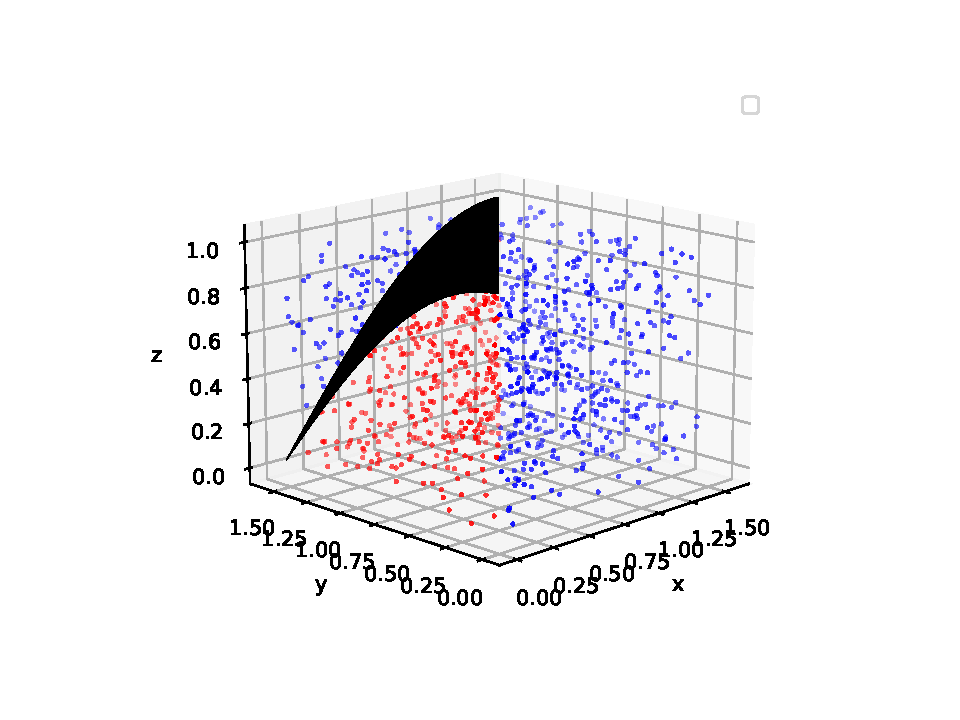
\includegraphics[width=0.78\textwidth]{img/graf.pdf}
    \end{center}
  \end{block}

  \vskip1.5ex

  % 5. a 6. Blok: Výběrové odhady a porovnání s teorií
  \begin{block}{5. a 6. Výběrové odhady a porovnání ($N = 1\,000$ pokusů)}
    \begin{table}
      \centering
      \small
      \begin{tabular}{lccc}
        \toprule
        \textbf{Charakteristika} & \textbf{Teoretická hodnota} & \textbf{Výběrový odhad} & \textbf{95\% Interval spolehlivosti} \\
        \midrule
        $E(X)$ & $0{,}5708$ & $0{,}5768$ & $[0{,}5388;\, 0{,}6149]$ \\
        $E(Y)$ & $1{,}0000$ & $1{,}0059$ & $[0{,}9674;\, 1{,}0444]$ \\
        $\operatorname{var}(X)$ & $0{,}1416$ & $0{,}1529$ & — \\
        $\operatorname{var}(Y)$ & $0{,}1416$ & $0{,}1562$ & — \\
        $\operatorname{cov}(X, Y)$ & $0{,}0921$ & $0{,}1002$ & — \\
        \bottomrule
      \end{tabular}
    \end{table}

    \begin{center}
      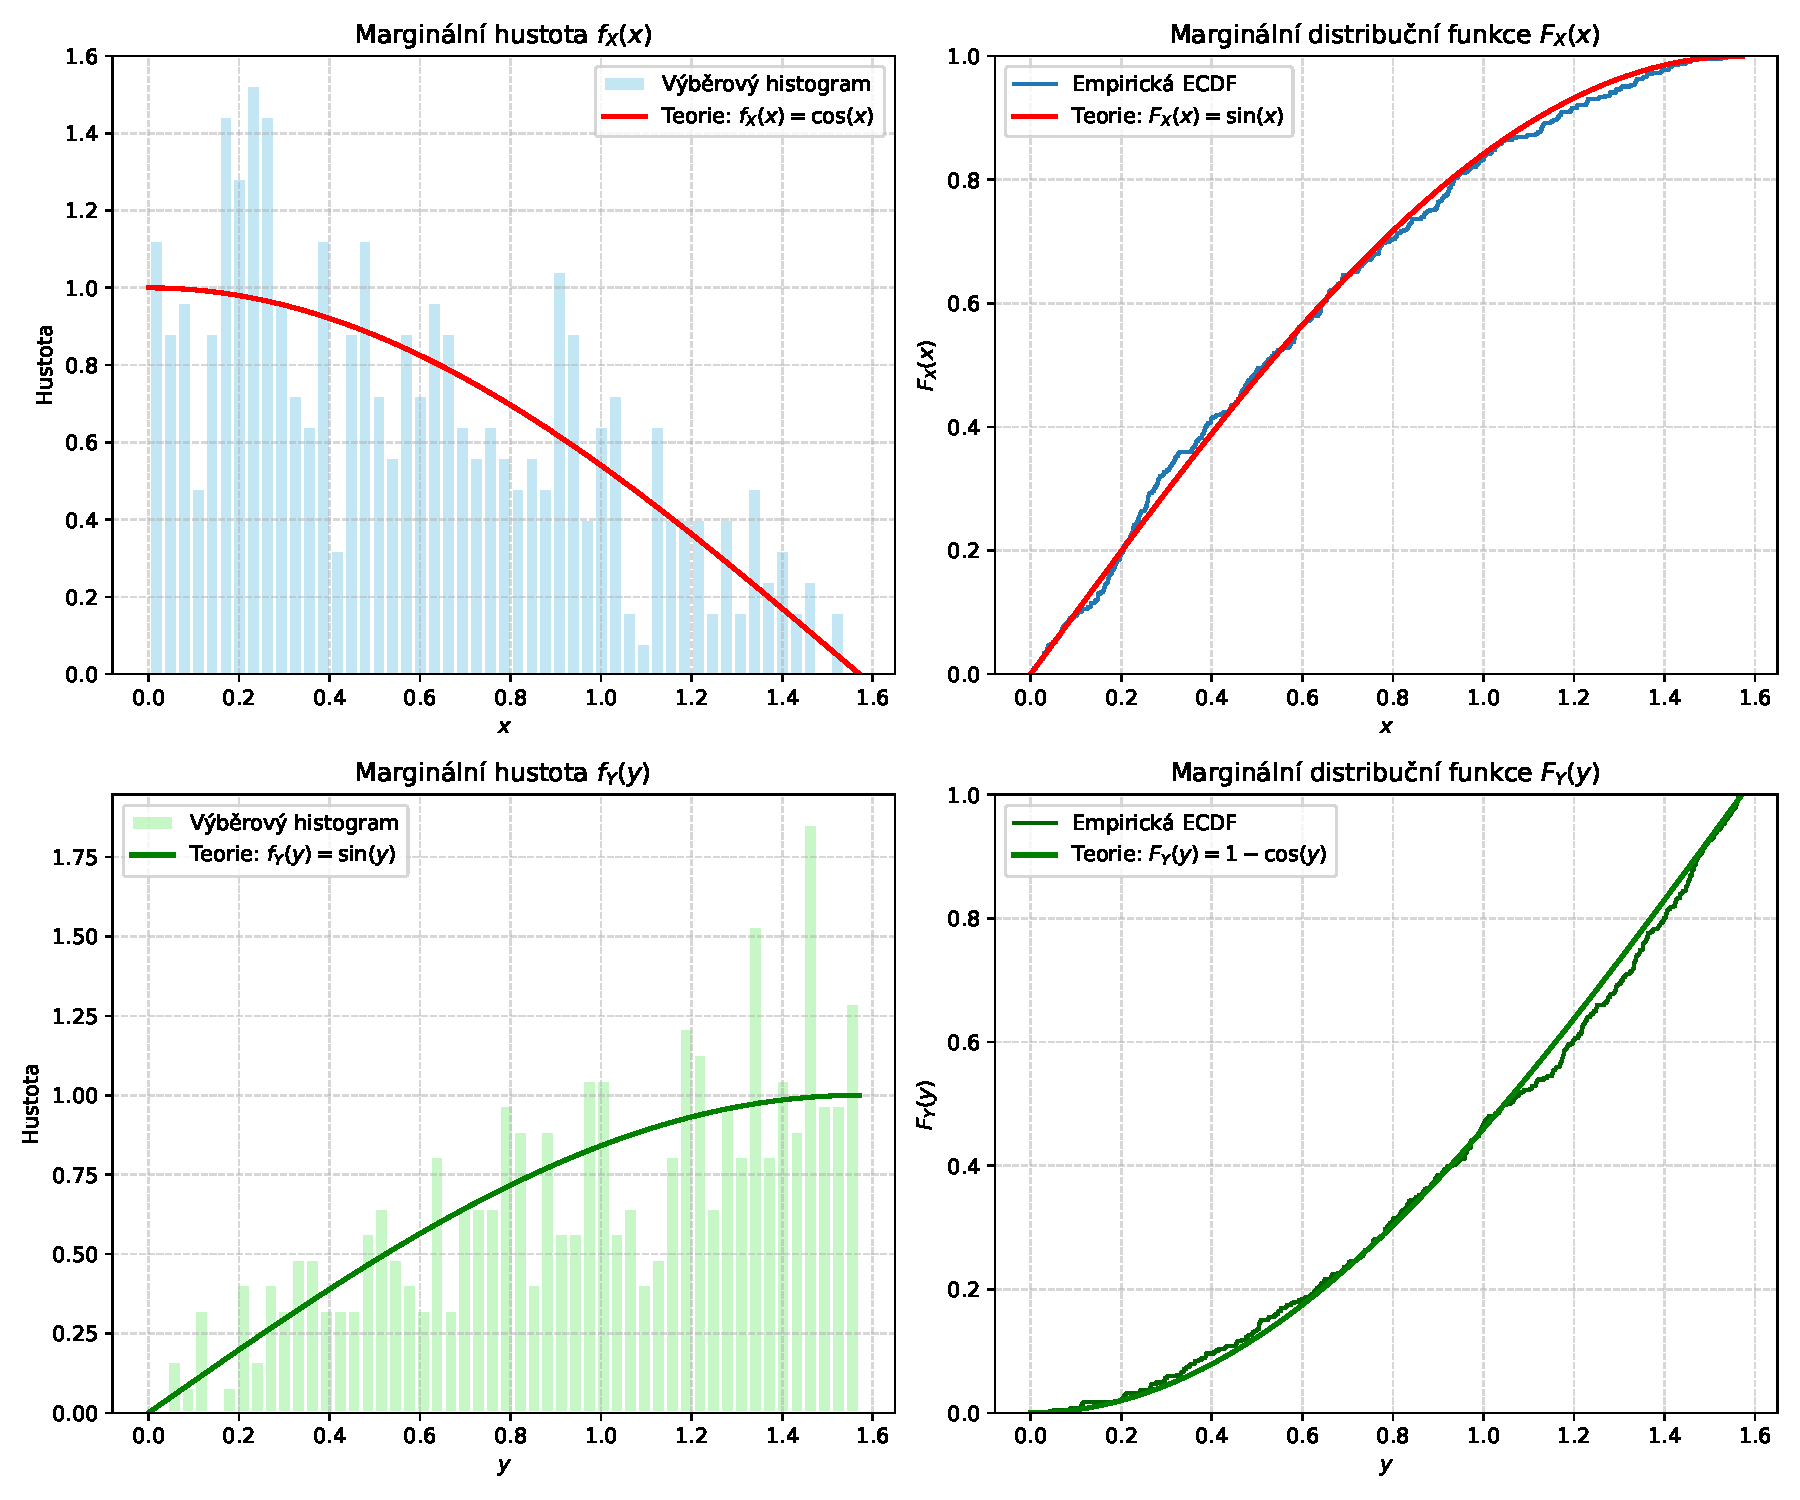
\includegraphics[width=0.88\textwidth]{img/histogramy.pdf}
    \end{center}
  \end{block}

  \vskip1.5ex

% 7. Blok: Závislost na rozsahu výběru
\begin{block}{7. Závislost přesnosti odhadu na rozsahu výběru ($n$)}
  Šířka oboustranného intervalu spolehlivosti
  $\Delta = 2 \cdot z_{1-\alpha/2} \cdot \frac{S}{\sqrt{n}}$
  konverguje k nule s rychlostí $\mathcal{O}(n^{-1/2})$:

  \begin{center}
    \small
    \setlength{\tabcolsep}{3pt}

    \textbf{Náhodná veličina $X$}

    \medskip
    \begin{tabular}{r@{\hspace{1cm}}ccc}
      \toprule
      \textbf{Rozsah výběru $n$}
      & $\bar{x}$
      & Chyba $|E(X) - \bar{x}|$
      & Šířka 95\% IS ($E(X)$) \\
      \midrule
      $100$         & $0{,}5474$ & $0{,}0234$ & $0{,}1419$ \\
      $1\,000$      & $0{,}5527$ & $0{,}0181$ & $0{,}0454$ \\
      $10\,000$     & $0{,}5696$ & $0{,}0012$ & $0{,}0148$ \\
      $100\,000$    & $0{,}5711$ & $0{,}0003$ & $0{,}0047$ \\
      $1\,000\,000$ & $0{,}5711$ & $0{,}0003$ & $0{,}0015$ \\
      \bottomrule
    \end{tabular}

    \bigskip
    \textbf{Náhodná veličina $Y$}

    \medskip
    \begin{tabular}{r@{\hspace{1cm}}ccc}
      \toprule
      \textbf{Rozsah výběru $n$}
      & $\bar{y}$
      & Chyba $|E(Y) - \bar{y}|$
      & Šířka 95\% IS ($E(Y)$) \\
      \midrule
      $100$         & $0{,}9528$ & $0{,}0472$ & $0{,}1477$ \\
      $1\,000$      & $0{,}9785$ & $0{,}0215$ & $0{,}0470$ \\
      $10\,000$     & $0{,}9991$ & $0{,}0009$ & $0{,}0148$ \\
      $100\,000$    & $0{,}9982$ & $0{,}0018$ & $0{,}0047$ \\
      $1\,000\,000$ & $0{,}9986$ & $0{,}0014$ & $0{,}0015$ \\
      \bottomrule
    \end{tabular}
  \end{center}

  Empirické marginální hustoty i ECDF z bodu 6 vykazují
  těsnou shodu se spočtenými teoretickými funkcemi
  $\cos(x)$, $\sin(y)$, $\sin(x)$ a $1 - \cos(y)$.
\end{block}

\end{column}

\end{columns}

\end{frame}
\end{document}